\documentclass[1p]{elsarticle_modified}
%\bibliographystyle{elsarticle-num}

%\usepackage[colorlinks]{hyperref}
%\usepackage{abbrmath_seonhwa} %\Abb, \Ascr, \Acal ,\Abf, \Afrak
\usepackage{amsfonts}
\usepackage{amssymb}
\usepackage{amsmath}
\usepackage{amsthm}
\usepackage{scalefnt}
\usepackage{amsbsy}
\usepackage{kotex}
\usepackage{caption}
\usepackage{subfig}
\usepackage{color}
\usepackage{graphicx}
\usepackage{xcolor} %% white, black, red, green, blue, cyan, magenta, yellow
\usepackage{float}
\usepackage{setspace}
\usepackage{hyperref}

\usepackage{tikz}
\usetikzlibrary{arrows}

\usepackage{multirow}
\usepackage{array} % fixed length table
\usepackage{hhline}

%%%%%%%%%%%%%%%%%%%%%
\makeatletter
\renewcommand*\env@matrix[1][\arraystretch]{%
	\edef\arraystretch{#1}%
	\hskip -\arraycolsep
	\let\@ifnextchar\new@ifnextchar
	\array{*\c@MaxMatrixCols c}}
\makeatother %https://tex.stackexchange.com/questions/14071/how-can-i-increase-the-line-spacing-in-a-matrix
%%%%%%%%%%%%%%%

\usepackage[normalem]{ulem}

\newcommand{\msout}[1]{\ifmmode\text{\sout{\ensuremath{#1}}}\else\sout{#1}\fi}
%SOURCE: \msout is \stkout macro in https://tex.stackexchange.com/questions/20609/strikeout-in-math-mode

\newcommand{\cancel}[1]{
	\ifmmode
	{\color{red}\msout{#1}}
	\else
	{\color{red}\sout{#1}}
	\fi
}

\newcommand{\add}[1]{
	{\color{blue}\uwave{#1}}
}

\newcommand{\replace}[2]{
	\ifmmode
	{\color{red}\msout{#1}}{\color{blue}\uwave{#2}}
	\else
	{\color{red}\sout{#1}}{\color{blue}\uwave{#2}}
	\fi
}

\newcommand{\Sol}{\mathcal{S}} %segment
\newcommand{\D}{D} %diagram
\newcommand{\A}{\mathcal{A}} %arc


%%%%%%%%%%%%%%%%%%%%%%%%%%%%%5 test

\def\sl{\operatorname{\textup{SL}}(2,\Cbb)}
\def\psl{\operatorname{\textup{PSL}}(2,\Cbb)}
\def\quan{\mkern 1mu \triangleright \mkern 1mu}

\theoremstyle{definition}
\newtheorem{thm}{Theorem}[section]
\newtheorem{prop}[thm]{Proposition}
\newtheorem{lem}[thm]{Lemma}
\newtheorem{ques}[thm]{Question}
\newtheorem{cor}[thm]{Corollary}
\newtheorem{defn}[thm]{Definition}
\newtheorem{exam}[thm]{Example}
\newtheorem{rmk}[thm]{Remark}
\newtheorem{alg}[thm]{Algorithm}

\newcommand{\I}{\sqrt{-1}}
\begin{document}

%\begin{frontmatter}
%
%\title{Boundary parabolic representations of knots up to 8 crossings}
%
%%% Group authors per affiliation:
%\author{Yunhi Cho} 
%\address{Department of Mathematics, University of Seoul, Seoul, Korea}
%\ead{yhcho@uos.ac.kr}
%
%
%\author{Seonhwa Kim} %\fnref{s_kim}}
%\address{Center for Geometry and Physics, Institute for Basic Science, Pohang, 37673, Korea}
%\ead{ryeona17@ibs.re.kr}
%
%\author{Hyuk Kim}
%\address{Department of Mathematical Sciences, Seoul National University, Seoul 08826, Korea}
%\ead{hyukkim@snu.ac.kr}
%
%\author{Seokbeom Yoon}
%\address{Department of Mathematical Sciences, Seoul National University, Seoul, 08826,  Korea}
%\ead{sbyoon15@snu.ac.kr}
%
%\begin{abstract}
%We find all boundary parabolic representation of knots up to 8 crossings.
%
%\end{abstract}
%\begin{keyword}
%    \MSC[2010] 57M25 
%\end{keyword}
%
%\end{frontmatter}

%\linenumbers
%\tableofcontents
%
\newcommand\colored[1]{\textcolor{white}{\rule[-0.35ex]{0.8em}{1.4ex}}\kern-0.8em\color{red} #1}%
%\newcommand\colored[1]{\textcolor{white}{ #1}\kern-2.17ex	\textcolor{white}{ #1}\kern-1.81ex	\textcolor{white}{ #1}\kern-2.15ex\color{red}#1	}

{\Large $\underline{9_{31}~(K9a_{13})}$}

\setlength{\tabcolsep}{10pt}
\renewcommand{\arraystretch}{1.6}
\vspace{1cm}\begin{tabular}{m{100pt}>{\centering\arraybackslash}m{274pt}}
\multirow{5}{120pt}{
	\centering
	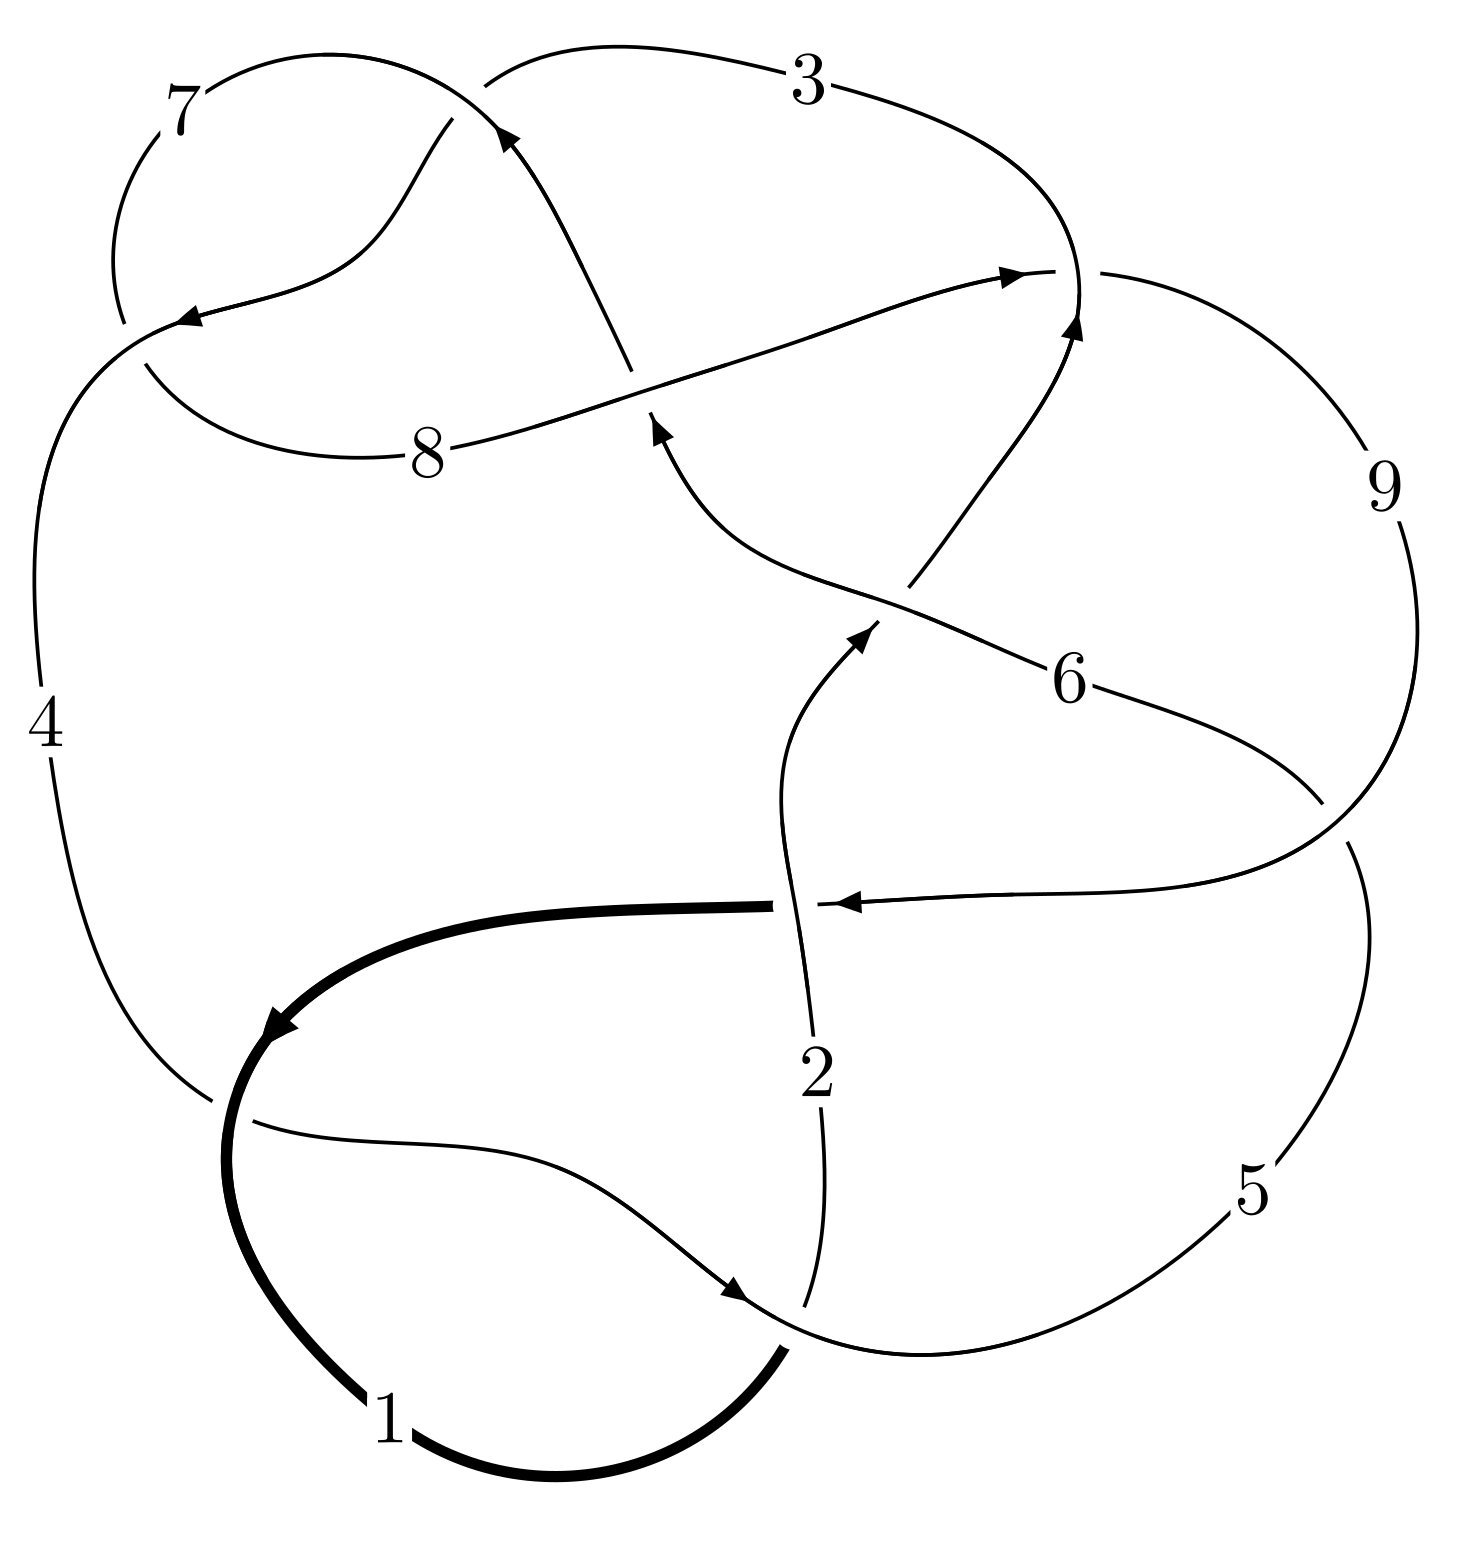
\includegraphics[width=112pt]{../../../GIT/diagram.site/Diagrams/png/66_9_31.png}\\
\ \ \ A knot diagram\footnotemark}&
\allowdisplaybreaks
\textbf{Linearized knot diagam} \\
\cline{2-2}
 &
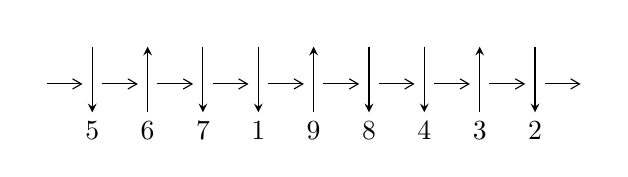
\begin{tikzpicture}[x=20pt, y=17pt]
	% nodes
	\node (C0) at (0, 0) {};
	\node (C1) at (1, 0) {};
	\node (C1U) at (1, +1) {};
	\node (C1D) at (1, -1) {5};

	\node (C2) at (2, 0) {};
	\node (C2U) at (2, +1) {};
	\node (C2D) at (2, -1) {6};

	\node (C3) at (3, 0) {};
	\node (C3U) at (3, +1) {};
	\node (C3D) at (3, -1) {7};

	\node (C4) at (4, 0) {};
	\node (C4U) at (4, +1) {};
	\node (C4D) at (4, -1) {1};

	\node (C5) at (5, 0) {};
	\node (C5U) at (5, +1) {};
	\node (C5D) at (5, -1) {9};

	\node (C6) at (6, 0) {};
	\node (C6U) at (6, +1) {};
	\node (C6D) at (6, -1) {8};

	\node (C7) at (7, 0) {};
	\node (C7U) at (7, +1) {};
	\node (C7D) at (7, -1) {4};

	\node (C8) at (8, 0) {};
	\node (C8U) at (8, +1) {};
	\node (C8D) at (8, -1) {3};

	\node (C9) at (9, 0) {};
	\node (C9U) at (9, +1) {};
	\node (C9D) at (9, -1) {2};
	\node (C10) at (10, 0) {};

	% arrows
	\draw[->,>={angle 60}]
	(C0) edge (C1) (C1) edge (C2) (C2) edge (C3) (C3) edge (C4) (C4) edge (C5) (C5) edge (C6) (C6) edge (C7) (C7) edge (C8) (C8) edge (C9) (C9) edge (C10) ;	\draw[->,>=stealth]
	(C1U) edge (C1D) (C2D) edge (C2U) (C3U) edge (C3D) (C4U) edge (C4D) (C5D) edge (C5U) (C6U) edge (C6D) (C7U) edge (C7D) (C8D) edge (C8U) (C9U) edge (C9D) ;
	\end{tikzpicture} \\
\hhline{~~} \\& 
\textbf{Solving Sequence} \\ \cline{2-2} 
 &
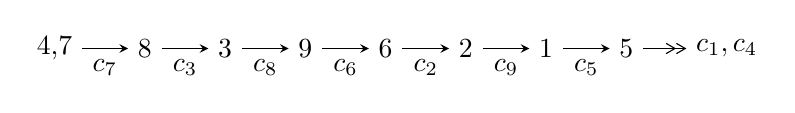
\begin{tikzpicture}[x=29pt, y=7pt]
	% node
	\node (A0) at (-1/8, 0) {4,7};
	\node (A1) at (1, 0) {8};
	\node (A2) at (2, 0) {3};
	\node (A3) at (3, 0) {9};
	\node (A4) at (4, 0) {6};
	\node (A5) at (5, 0) {2};
	\node (A6) at (6, 0) {1};
	\node (A7) at (7, 0) {5};
	\node (C1) at (1/2, -1) {$c_{7}$};
	\node (C2) at (3/2, -1) {$c_{3}$};
	\node (C3) at (5/2, -1) {$c_{8}$};
	\node (C4) at (7/2, -1) {$c_{6}$};
	\node (C5) at (9/2, -1) {$c_{2}$};
	\node (C6) at (11/2, -1) {$c_{9}$};
	\node (C7) at (13/2, -1) {$c_{5}$};
	\node (A8) at (33/4, 0) {$c_{1},c_{4}$};

	% edge
	\draw[->,>=stealth]	
	(A0) edge (A1) (A1) edge (A2) (A2) edge (A3) (A3) edge (A4) (A4) edge (A5) (A5) edge (A6) (A6) edge (A7) ;
	\draw[->>,>={angle 60}]	
	(A7) edge (A8);
\end{tikzpicture} \\ 

\end{tabular} \\

\footnotetext{
The image of knot diagram is generated by the software ``\textbf{Draw programme}" developed by Andrew Bartholomew(\url{http://www.layer8.co.uk/maths/draw/index.htm\#Running-draw}), where we modified some parts for our purpose(\url{https://github.com/CATsTAILs/LinksPainter}).
}\phantom \\ \newline 
\centering \textbf{Ideals for irreducible components\footnotemark of $X_{\text{par}}$} 
 
\begin{align*}
I^u_{1}&=\langle 
u^7-2 u^5+2 u^3- u^2+1\rangle \\
I^u_{2}&=\langle 
u^{20}+u^{19}+\cdots+2 u+1\rangle \\
\\
\end{align*}
\raggedright * 2 irreducible components of $\dim_{\mathbb{C}}=0$, with total 27 representations.\\
\footnotetext{All coefficients of polynomials are rational numbers. But the coefficients are sometimes approximated in decimal forms when there is not enough margin.}
\newpage
\renewcommand{\arraystretch}{1}
\centering \section*{I. $I^u_{1}= \langle u^7-2 u^5+2 u^3- u^2+1 \rangle$}
\flushleft \textbf{(i) Arc colorings}\\
\begin{tabular}{m{7pt} m{180pt} m{7pt} m{180pt} }
\flushright $a_{4}=$&$\begin{pmatrix}0\\u\end{pmatrix}$ \\
\flushright $a_{7}=$&$\begin{pmatrix}1\\0\end{pmatrix}$ \\
\flushright $a_{8}=$&$\begin{pmatrix}1\\u^2\end{pmatrix}$ \\
\flushright $a_{3}=$&$\begin{pmatrix}u\\u\end{pmatrix}$ \\
\flushright $a_{9}=$&$\begin{pmatrix}u^4- u^2+1\\u^4\end{pmatrix}$ \\
\flushright $a_{6}=$&$\begin{pmatrix}- u^2+1\\- u^4\end{pmatrix}$ \\
\flushright $a_{2}=$&$\begin{pmatrix}u^2-1\\u^5+u^4-2 u^3+u-1\end{pmatrix}$ \\
\flushright $a_{1}=$&$\begin{pmatrix}1\\- u^6+u^4+u^3+1\end{pmatrix}$ \\
\flushright $a_{5}=$&$\begin{pmatrix}- u\\u^5- u^4-2 u^3+u^2-1\end{pmatrix}$\\ \flushright $a_{5}=$&$\begin{pmatrix}- u\\u^5- u^4-2 u^3+u^2-1\end{pmatrix}$\\&\end{tabular}
\flushleft \textbf{(ii) Obstruction class $= -1$}\\~\\
\flushleft \textbf{(iii) Cusp Shapes $= 4 u^5+4 u^4-8 u^3-4 u^2+4 u-6$}\\~\\
\newpage\renewcommand{\arraystretch}{1}
\flushleft \textbf{(iv) u-Polynomials at the component}\newline \\
\begin{tabular}{m{50pt}|m{274pt}}
Crossings & \hspace{64pt}u-Polynomials at each crossing \\
\hline $$\begin{aligned}c_{1},c_{3},c_{4}\\c_{7}\end{aligned}$$&$\begin{aligned}
&u^7-2 u^5+2 u^3- u^2+1
\end{aligned}$\\
\hline $$\begin{aligned}c_{2}\end{aligned}$$&$\begin{aligned}
&u^7-5 u^6+12 u^5-17 u^4+15 u^3-5 u^2-4 u+4
\end{aligned}$\\
\hline $$\begin{aligned}c_{5},c_{8}\end{aligned}$$&$\begin{aligned}
&u^7+2 u^5-2 u^4+4 u^3- u^2+2 u+1
\end{aligned}$\\
\hline $$\begin{aligned}c_{6},c_{9}\end{aligned}$$&$\begin{aligned}
&u^7+4 u^6+8 u^5+8 u^4+4 u^3+u^2+2 u+1
\end{aligned}$\\
\hline
\end{tabular}\\~\\
\newpage\renewcommand{\arraystretch}{1}
\flushleft \textbf{(v) Riley Polynomials at the component}\newline \\
\begin{tabular}{m{50pt}|m{274pt}}
Crossings & \hspace{64pt}Riley Polynomials at each crossing \\
\hline $$\begin{aligned}c_{1},c_{3},c_{4}\\c_{7}\end{aligned}$$&$\begin{aligned}
&y^7-4 y^6+8 y^5-8 y^4+4 y^3- y^2+2 y-1
\end{aligned}$\\
\hline $$\begin{aligned}c_{2}\end{aligned}$$&$\begin{aligned}
&y^7- y^6+4 y^5+13 y^4- y^3-9 y^2+56 y-16
\end{aligned}$\\
\hline $$\begin{aligned}c_{5},c_{8}\end{aligned}$$&$\begin{aligned}
&y^7+4 y^6+12 y^5+16 y^4+20 y^3+19 y^2+6 y-1
\end{aligned}$\\
\hline $$\begin{aligned}c_{6},c_{9}\end{aligned}$$&$\begin{aligned}
&y^7+8 y^5-4 y^4+24 y^3- y^2+2 y-1
\end{aligned}$\\
\hline
\end{tabular}\\~\\
\newpage\flushleft \textbf{(vi) Complex Volumes and Cusp Shapes}
$$\begin{array}{c|c|c}  
\text{Solutions to }I^u_{1}& \I (\text{vol} + \sqrt{-1}CS) & \text{Cusp shape}\\
 \hline 
\begin{aligned}
u &= \phantom{-}1.125110 + 0.343189 I\end{aligned}
 & -5.94607 - 3.76357 I & -10.60460 + 4.24459 I \\ \hline\begin{aligned}
u &= \phantom{-}1.125110 - 0.343189 I\end{aligned}
 & -5.94607 + 3.76357 I & -10.60460 - 4.24459 I \\ \hline\begin{aligned}
u &= \phantom{-}0.364544 + 0.701794 I\end{aligned}
 & \phantom{-}1.82567 + 1.84683 I & \phantom{-}1.12815 - 1.09324 I \\ \hline\begin{aligned}
u &= \phantom{-}0.364544 - 0.701794 I\end{aligned}
 & \phantom{-}1.82567 - 1.84683 I & \phantom{-}1.12815 + 1.09324 I \\ \hline\begin{aligned}
u &= -1.125830 + 0.566290 I\end{aligned}
 & -2.65707 + 11.68630 I & -5.70307 - 8.84509 I \\ \hline\begin{aligned}
u &= -1.125830 - 0.566290 I\end{aligned}
 & -2.65707 - 11.68630 I & -5.70307 + 8.84509 I \\ \hline\begin{aligned}
u &= -0.727635\phantom{ +0.000000I}\end{aligned}
 & -1.24946\phantom{ +0.000000I} & -7.64100\phantom{ +0.000000I}\\
 \hline 
 \end{array}$$\newpage\newpage\renewcommand{\arraystretch}{1}
\centering \section*{II. $I^u_{2}= \langle u^{20}+u^{19}-4 u^{18}-5 u^{17}+8 u^{16}+13 u^{15}-7 u^{14}-20 u^{13}- u^{12}+19 u^{11}+10 u^{10}-10 u^9-11 u^8+2 u^7+7 u^6+u^5-3 u^4- u^3+2 u^2+2 u+1 \rangle$}
\flushleft \textbf{(i) Arc colorings}\\
\begin{tabular}{m{7pt} m{180pt} m{7pt} m{180pt} }
\flushright $a_{4}=$&$\begin{pmatrix}0\\u\end{pmatrix}$ \\
\flushright $a_{7}=$&$\begin{pmatrix}1\\0\end{pmatrix}$ \\
\flushright $a_{8}=$&$\begin{pmatrix}1\\u^2\end{pmatrix}$ \\
\flushright $a_{3}=$&$\begin{pmatrix}u\\u\end{pmatrix}$ \\
\flushright $a_{9}=$&$\begin{pmatrix}u^4- u^2+1\\u^4\end{pmatrix}$ \\
\flushright $a_{6}=$&$\begin{pmatrix}- u^2+1\\- u^4\end{pmatrix}$ \\
\flushright $a_{2}=$&$\begin{pmatrix}u^7-2 u^5+2 u^3\\u^9- u^7+u^5+u\end{pmatrix}$ \\
\flushright $a_{1}=$&$\begin{pmatrix}- u^{19}- u^{18}+\cdots-3 u^2-2 u\\u^{11}-3 u^9+4 u^7-3 u^5+u^3- u-1\end{pmatrix}$ \\
\flushright $a_{5}=$&$\begin{pmatrix}u^{12}-3 u^{10}+5 u^8-4 u^6+2 u^4- u^2+1\\u^{12}-2 u^{10}+2 u^8- u^4\end{pmatrix}$\\ \flushright $a_{5}=$&$\begin{pmatrix}u^{12}-3 u^{10}+5 u^8-4 u^6+2 u^4- u^2+1\\u^{12}-2 u^{10}+2 u^8- u^4\end{pmatrix}$\\&\end{tabular}
\flushleft \textbf{(ii) Obstruction class $= -1$}\\~\\
\flushleft \textbf{(iii) Cusp Shapes $= 4 u^{18}-16 u^{16}+36 u^{14}-48 u^{12}+44 u^{10}-28 u^8-4 u^7+16 u^6+8 u^5-8 u^4-8 u^3+4 u^2+4 u-2$}\\~\\
\newpage\renewcommand{\arraystretch}{1}
\flushleft \textbf{(iv) u-Polynomials at the component}\newline \\
\begin{tabular}{m{50pt}|m{274pt}}
Crossings & \hspace{64pt}u-Polynomials at each crossing \\
\hline $$\begin{aligned}c_{1},c_{3},c_{4}\\c_{7}\end{aligned}$$&$\begin{aligned}
&u^{20}+u^{19}+\cdots+2 u+1
\end{aligned}$\\
\hline $$\begin{aligned}c_{2}\end{aligned}$$&$\begin{aligned}
&(u^{10}+2 u^9+u^8+4 u^6+6 u^5+u^4-6 u^3-5 u^2+1)^2
\end{aligned}$\\
\hline $$\begin{aligned}c_{5},c_{8}\end{aligned}$$&$\begin{aligned}
&u^{20}+3 u^{19}+\cdots+16 u+5
\end{aligned}$\\
\hline $$\begin{aligned}c_{6},c_{9}\end{aligned}$$&$\begin{aligned}
&u^{20}+9 u^{19}+\cdots+2 u^2+1
\end{aligned}$\\
\hline
\end{tabular}\\~\\
\newpage\renewcommand{\arraystretch}{1}
\flushleft \textbf{(v) Riley Polynomials at the component}\newline \\
\begin{tabular}{m{50pt}|m{274pt}}
Crossings & \hspace{64pt}Riley Polynomials at each crossing \\
\hline $$\begin{aligned}c_{1},c_{3},c_{4}\\c_{7}\end{aligned}$$&$\begin{aligned}
&y^{20}-9 y^{19}+\cdots+2 y^2+1
\end{aligned}$\\
\hline $$\begin{aligned}c_{2}\end{aligned}$$&$\begin{aligned}
&(y^{10}-2 y^9+\cdots-10 y+1)^{2}
\end{aligned}$\\
\hline $$\begin{aligned}c_{5},c_{8}\end{aligned}$$&$\begin{aligned}
&y^{20}+3 y^{19}+\cdots+204 y+25
\end{aligned}$\\
\hline $$\begin{aligned}c_{6},c_{9}\end{aligned}$$&$\begin{aligned}
&y^{20}+3 y^{19}+\cdots+4 y+1
\end{aligned}$\\
\hline
\end{tabular}\\~\\
\newpage\flushleft \textbf{(vi) Complex Volumes and Cusp Shapes}
$$\begin{array}{c|c|c}  
\text{Solutions to }I^u_{2}& \I (\text{vol} + \sqrt{-1}CS) & \text{Cusp shape}\\
 \hline 
\begin{aligned}
u &= -0.941429 + 0.547698 I\end{aligned}
 & \phantom{-}0.197299\phantom{ +0.000000I} & -2.26625 + 0. I\phantom{ +0.000000I} \\ \hline\begin{aligned}
u &= -0.941429 - 0.547698 I\end{aligned}
 & \phantom{-}0.197299\phantom{ +0.000000I} & -2.26625 + 0. I\phantom{ +0.000000I} \\ \hline\begin{aligned}
u &= -1.061040 + 0.273586 I\end{aligned}
 & -2.27340 + 0.51998 I & -5.71661 - 0.77505 I \\ \hline\begin{aligned}
u &= -1.061040 - 0.273586 I\end{aligned}
 & -2.27340 - 0.51998 I & -5.71661 + 0.77505 I \\ \hline\begin{aligned}
u &= -0.626658 + 0.633601 I\end{aligned}
 & \phantom{-}1.11960 + 4.65452 I & -0.79654 - 6.04247 I \\ \hline\begin{aligned}
u &= -0.626658 - 0.633601 I\end{aligned}
 & \phantom{-}1.11960 - 4.65452 I & -0.79654 + 6.04247 I \\ \hline\begin{aligned}
u &= \phantom{-}1.128770 + 0.240119 I\end{aligned}
 & -4.83313 + 3.92983 I & -9.04400 - 3.21471 I \\ \hline\begin{aligned}
u &= \phantom{-}1.128770 - 0.240119 I\end{aligned}
 & -4.83313 - 3.92983 I & -9.04400 + 3.21471 I \\ \hline\begin{aligned}
u &= \phantom{-}1.016360 + 0.552370 I\end{aligned}
 & \phantom{-}1.11960 - 4.65452 I & -0.79654 + 6.04247 I \\ \hline\begin{aligned}
u &= \phantom{-}1.016360 - 0.552370 I\end{aligned}
 & \phantom{-}1.11960 + 4.65452 I & -0.79654 - 6.04247 I \\ \hline\begin{aligned}
u &= -0.330984 + 0.758157 I\end{aligned}
 & -0.32496 - 6.68616 I & -2.49331 + 5.21994 I \\ \hline\begin{aligned}
u &= -0.330984 - 0.758157 I\end{aligned}
 & -0.32496 + 6.68616 I & -2.49331 - 5.21994 I \\ \hline\begin{aligned}
u &= \phantom{-}0.527984 + 0.630206 I\end{aligned}
 & \phantom{-}2.55688\phantom{ +0.000000I} & \phantom{-}2.36717 + 0. I\phantom{ +0.000000I} \\ \hline\begin{aligned}
u &= \phantom{-}0.527984 - 0.630206 I\end{aligned}
 & \phantom{-}2.55688\phantom{ +0.000000I} & \phantom{-}2.36717 + 0. I\phantom{ +0.000000I} \\ \hline\begin{aligned}
u &= -1.119570 + 0.508145 I\end{aligned}
 & -4.83313 + 3.92983 I & -9.04400 - 3.21471 I \\ \hline\begin{aligned}
u &= -1.119570 - 0.508145 I\end{aligned}
 & -4.83313 - 3.92983 I & -9.04400 + 3.21471 I \\ \hline\begin{aligned}
u &= \phantom{-}1.102100 + 0.557039 I\end{aligned}
 & -0.32496 - 6.68616 I & -2.49331 + 5.21994 I \\ \hline\begin{aligned}
u &= \phantom{-}1.102100 - 0.557039 I\end{aligned}
 & -0.32496 + 6.68616 I & -2.49331 - 5.21994 I \\ \hline\begin{aligned}
u &= -0.195538 + 0.653472 I\end{aligned}
 & -2.27340 + 0.51998 I & -5.71661 - 0.77505 I \\ \hline\begin{aligned}
u &= -0.195538 - 0.653472 I\end{aligned}
 & -2.27340 - 0.51998 I & -5.71661 + 0.77505 I\\
 \hline 
 \end{array}$$\newpage
\newpage\renewcommand{\arraystretch}{1}
\centering \section*{ III. u-Polynomials}
\begin{tabular}{m{50pt}|m{274pt}}
Crossings & \hspace{64pt}u-Polynomials at each crossing \\
\hline $$\begin{aligned}c_{1},c_{3},c_{4}\\c_{7}\end{aligned}$$&$\begin{aligned}
&(u^7-2 u^5+2 u^3- u^2+1)(u^{20}+u^{19}+\cdots+2 u+1)
\end{aligned}$\\
\hline $$\begin{aligned}c_{2}\end{aligned}$$&$\begin{aligned}
&(u^7-5 u^6+12 u^5-17 u^4+15 u^3-5 u^2-4 u+4)\\
&\cdot(u^{10}+2 u^9+u^8+4 u^6+6 u^5+u^4-6 u^3-5 u^2+1)^2
\end{aligned}$\\
\hline $$\begin{aligned}c_{5},c_{8}\end{aligned}$$&$\begin{aligned}
&(u^7+2 u^5-2 u^4+4 u^3- u^2+2 u+1)(u^{20}+3 u^{19}+\cdots+16 u+5)
\end{aligned}$\\
\hline $$\begin{aligned}c_{6},c_{9}\end{aligned}$$&$\begin{aligned}
&(u^7+4 u^6+\cdots+2 u+1)(u^{20}+9 u^{19}+\cdots+2 u^2+1)
\end{aligned}$\\
\hline
\end{tabular}\newpage\renewcommand{\arraystretch}{1}
\centering \section*{ IV. Riley Polynomials}
\begin{tabular}{m{50pt}|m{274pt}}
Crossings & \hspace{64pt}Riley Polynomials at each crossing \\
\hline $$\begin{aligned}c_{1},c_{3},c_{4}\\c_{7}\end{aligned}$$&$\begin{aligned}
&(y^7-4 y^6+\cdots+2 y-1)(y^{20}-9 y^{19}+\cdots+2 y^2+1)
\end{aligned}$\\
\hline $$\begin{aligned}c_{2}\end{aligned}$$&$\begin{aligned}
&(y^7- y^6+4 y^5+13 y^4- y^3-9 y^2+56 y-16)\\
&\cdot(y^{10}-2 y^9+\cdots-10 y+1)^{2}
\end{aligned}$\\
\hline $$\begin{aligned}c_{5},c_{8}\end{aligned}$$&$\begin{aligned}
&(y^7+4 y^6+12 y^5+16 y^4+20 y^3+19 y^2+6 y-1)\\
&\cdot(y^{20}+3 y^{19}+\cdots+204 y+25)
\end{aligned}$\\
\hline $$\begin{aligned}c_{6},c_{9}\end{aligned}$$&$\begin{aligned}
&(y^7+8 y^5+\cdots+2 y-1)(y^{20}+3 y^{19}+\cdots+4 y+1)
\end{aligned}$\\
\hline
\end{tabular}
\vskip 2pc
\end{document}